\section{Extraction des informations}

	\begin{frame}
		\begin{itemize}
		\item Retour sur les données brutes
			\begin{itemize}
				\item \textit{The employee was welding overhead and the wind shifted, resulting in discomfort in eye.}\\
			\end{itemize}
		\item On cherche à connaître le niveau de risque de la situation et le potentiel d'escalation.
		\item Il s'agit d'un problème de régression classique d'apprentissage automatique.
		\end{itemize}			
	\end{frame}


\begin{frame}
	L'apprentissage automatique supervisé en général
	\begin{itemize}
		\item Soit n documents, ayant chacun une étiquette.
		\item l'algorithme d'apprentissaage automatique cherche à optimiser une fonction objective
		\item qui minimise les erreurs entre les intrants et leur réponse attendue
		\item afin de généraliser et d'avoir un pouvoir de prédiction
	\end{itemize}			
	
	\bigskip
	
	Dans le cas actuel
	\begin{itemize}
		\item Les données textuelles brutes sont difficile à utiliser.
		\item Non numérique, Non structurée 
		\item Étiquette étant le niveau de risque 	
	\end{itemize}			
\end{frame}


\begin{frame}
	Extraction d'information
	\begin{itemize}
		\item Parallèle existant entre la régression linéaire.
		\item Extraire les mots clés
		\item \cite{prades} et \cite{desvignes} ont analysé 2210 rapport d'accidents venant de 476 contracteyrs
		\item Solution optimale : 80 mots précurseurs et 5 catégories d'outcome
	\end{itemize}			
\end{frame}


\begin{frame}
	Précurseurs
	\begin{itemize}
		\item Mots libre de contexte.
		\item \textit{The employee was welding overhead and the wind shifted, resulting in discomfort in eye.}\\
		\begin{itemize}
			\item Welding, working overhead, Wind
		\end{itemize}
		
	
		\item Situation semblant très courtante sur un chantier de construction
	\end{itemize}	

		
\end{frame}


\begin{frame}
	Exemple de mot précurseurs\\
	
	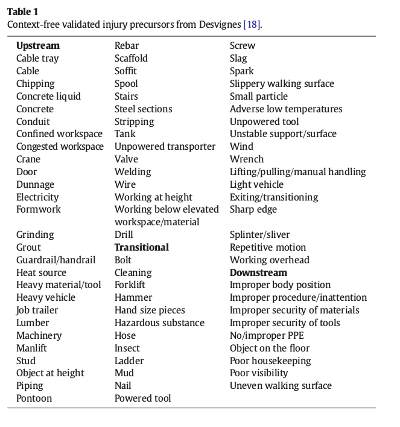
\includegraphics[width=\paperwidth]{table_precurseurs}
\end{frame}


\begin{frame}	
	L'attribution de ces mots clé est fait à la main par Prades et Davigne
	\begin{itemize}
		\item Ce n'est pas une approche qui est viable a long terme.		
		\item Il faut automatiser l'extraction de ces mots-clés.		
		\item On entraine un robot apprenant à faire cette tâche.
		\item On doit s'assurer que bien contrôler les intrants.
	\end{itemize}
\end{frame}


\begin{frame}	
	Le robot apprenant devra prétraiter les intrants afin de:
	\begin{itemize}
		\item Reconnaître les différentes formes d'un même mot.		
		\item Faire la différence contextuelle de l'utilisation d'un mot.		
	\end{itemize}
	Puis extraire les bons précurseurs à l'aide d'un :
	\begin{itemize}
		\item Lexique pour entreposer les mots qu'il connait, 		
		\item Ensemble de règle connecntant des "groupes syntaxiques" vers un précurseur.		
	\end{itemize}
\end{frame}


\begin{frame}
	Reconnaître les différentes forme d'un même mot
	\begin{itemize}
		\item Les mots ne sont pas toujours écrit de la même façon
		\item \textit{Worker is unloading a ladder from pickup with bad posture.}\\
		\begin{itemize}
			\item Ladder, Manual handling, Light vehicule, Improper body positionning
		\end{itemize}
		\item On veux aussi considérer les déclinaisons des mots
		\begin{itemize}
			\item Ladder vs ladders, unloading vs unloads ...
		\end{itemize}
		\item Il est important de normaliser les mots, tout en gardant un sens dans le contexte.
	\end{itemize}
\end{frame}



\begin{frame}
	Normalisation des mots
	\begin{itemize}
		\item Analyse morphologique (Connassaince de la langue)
		\begin{itemize}
			\item Beau, Magifnique, Joli ...
		\end{itemize}	
		\item Lemmatisation (Utilisation d'un lexique)
		\begin{itemize}
			\item Beau, Beaux, Belle, Belles ...
		\end{itemize}	
		\item Racinisation (Ensemble de règles)
		\begin{itemize}
			\item Beau -> Bel, Beaux -> Bel, Belle -> Bel, Belles ...
			\item Organisation -> Organ, Organe -> Organ
		\end{itemize}	
		
	\end{itemize}
\end{frame}

\begin{frame}	
	Différencier l'utilisation de mots dépendant du contexte
	\begin{itemize}
		\item \textit{Moving floor plate, employee strained his back.}\\
		\item \textit{Employee rolled his angle on moving floor plate.}\\
	\end{itemize}
	Moving floor plate est exactement le même mot, mais clairement les deux mots clés associés ne seront pas les mêmes
	\begin{itemize}
		\item Verbe déplacer : Manual Handling\\
		\item Adjectif mobile : Unstable Surface\\
	\end{itemize}	
\end{frame}

\begin{frame}	
	POS - Part of Speach tagging
	\begin{itemize}
		\item Affecter le bon type lexical au bon mot
		\item Utilisation des chaînes de Markov cachées (HMM)
		\item On cherche à résoudre l'équation suivante
		\begin{itemize}
			\item $\textrm{argmax}_{t^1}  \prod_{i=1}^{n}  P(W_i|t_i) P(t_i|t_{i-1}) $
			\item Pour tous les mots de la phrase, en même temps.
			\item Problème NP complexe - utilisation possible de la programmation dynamique.
		\end{itemize}
	\end{itemize}
	Dans l'article ils ont utiliés les mots de préposition pour inférer le type lexical au lieu d'ajouter des l'information aux intrants.
\end{frame}

\begin{frame}	
	Modèle de n-gram
	\begin{itemize}
		\item Une entité textuelle n'est pas nécessairement un seul mot
		\item Extraire des groupes de mots pour lequels un sens est ajouté lorsque combiné
		\begin{itemize}
			\item Concrete floor : Concrete
			\item Concrete drill : Powered Tool
			\item Concrete burn : Concrete liquid 
			\item Concrete bag : Heavy Material
		\end{itemize}	
	\end{itemize}
	On enrichi le lexique des groupes avec ces n-grams.
\end{frame}

\begin{frame}	
	Framework de la création de l'outil d'extraction (NER)
	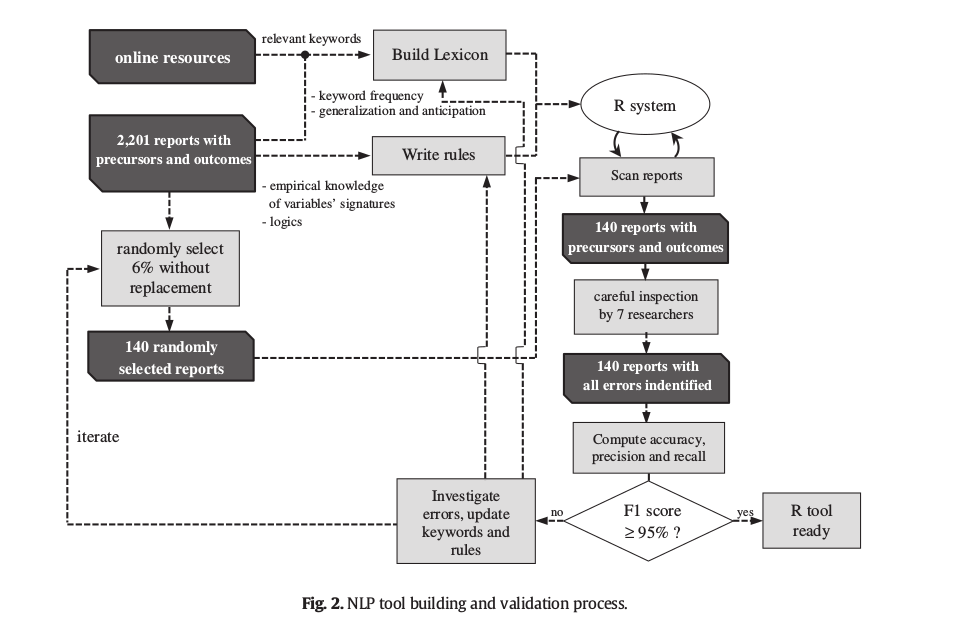
\includegraphics[width=\paperwidth]{rtool_training_framework}
\end{frame}



\begin{frame}	
	
	Métriques de qualité de prédiction\\
	- Précision : la précision est la capacité d'un classifieur à ne trouver que les données d'une classe en particulier. Minimise les faux positifs.	\begin{center}
		$\textrm{Précision} = \frac{\sum_{i=1}^{l} tp_i}{\sum_{i=1}^{l} (tp_i + fp_i)}$
	\end{center}
	
	- Rappel (sensibilité): le rappel est la capacité du classifieur à bien trouver toutes les données d'une classe en particulier. maximise les vrais positifs.
		\begin{center}
		$\textrm{Rappel} = \frac{\sum_{i=1}^{l} tp_i}{\sum_{i=1}^{l} (tp_i + fn_i)}$
	\end{center}
	
	- Score F: le score F est la moyenne harmonique de la précision et du rappel. 
	\begin{center}
		$\textrm{Score F} = \frac{2 * \textrm{Précision} * \textrm{Rappel}}{\textrm{Précision} + \textrm{Rappel}}$ 
	\end{center}
	
\end{frame}




\begin{frame}	
	Transformation d'un problème textuel en problème matriciel
	\begin{itemize}
		\item Automate permettant de transformer un texte libre en vecteur v tel que
		\item v(j) = 1 si le $\textrm{précurseur}_j$ a été trouvé, 0 autrement 
	\end{itemize}
	
	Et vers un problème d'apprentissage automatique
	\begin{itemize}
		\item Soit un jeu de données comprenant R rapports pouvant contenir P précurseurs
		\item On obtiens la matrice creuse $\textrm{RP}^{RxP}$
	\end{itemize}
\end{frame}



\begin{frame}	
	Outil d'extraction
	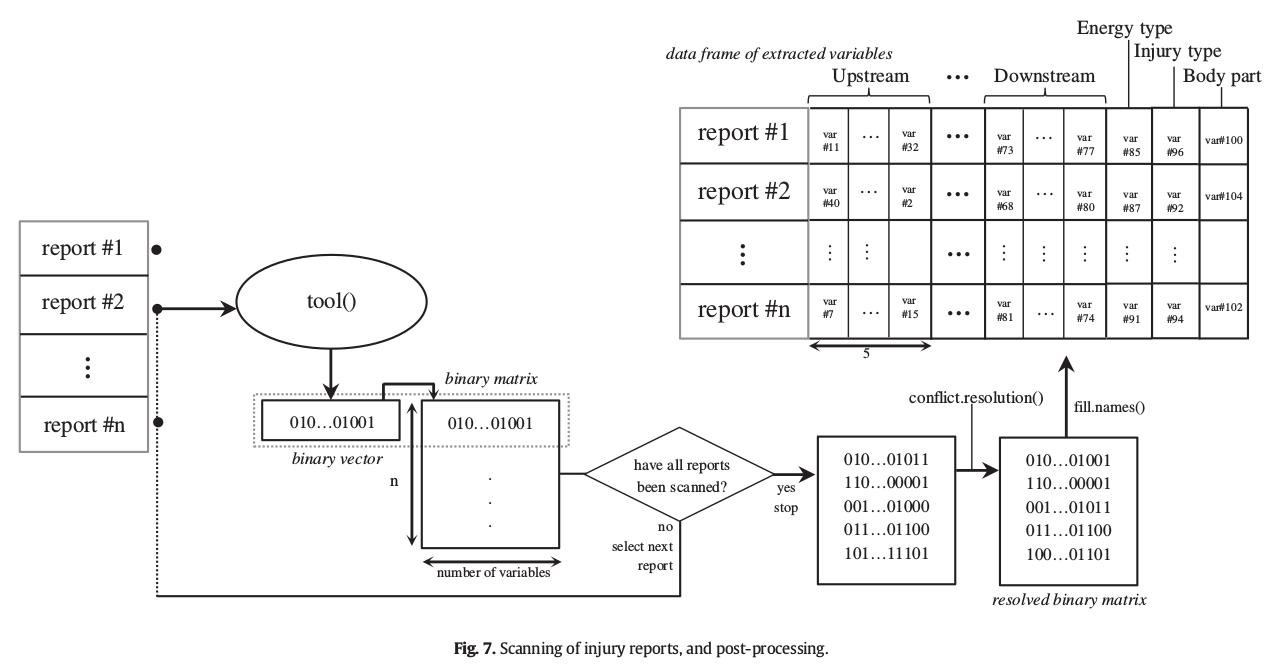
\includegraphics[width=\paperwidth]{rtool}
\end{frame}

\begin{frame}	
	Pipeline habituelle en traitement de la langue natuerelle
	
	\begin{itemize}
		\item Tokenisation - transformer les textes en matrice creuse
		\begin{itemize}
			\item Part of speach tagging
			\item Normalisation
			\item N-gram
		\end{itemize}
		
		\item Ponderation - mettre de l'emphase sur certains mots
		\begin{itemize}
			\item TF/IDF
			\item Separation Bi-Normale
		\end{itemize}
		
		\item Calibration d'un prédicteur - transférer les connaissance à la machine apprenante
		\begin{itemize}
			\item Utilisation d'une table de vérité, ou d'un oracle.
			\item SVM, Boosing, etc...
		\end{itemize}
		
	\end{itemize}
\end{frame}

\begin{frame}[t]
	
	Soit la matrice creuse RP suivante, \\
	\begin{tabular}[t]{lcccc}
		rapport & $w_1$ & $w_2$ & ... & $w_p$ \\
		$\textrm{rapport}_1$ & 1 & 0 &  & 1 \\
		$\textrm{rapport}_2$ & 1 & 0 &  & 1 \\
		$\textrm{rapport}_3$ & 0 & 1 &  & 1 \\
		... &  &  &  & \\
		$\textrm{rapport}_R$ & 1 & 1 &  & 1 \\
	\end{tabular}\\
	\bigskip
	On a la transformation TF-IDF. Cette transformation pénalise les mots qui sont utilisés dans beaucoup de documents\\
	\bigskip
	
	$RP(r, p) = RP(r, p) * \textrm{td-idf}(w_p, d, n_w, r)$, avec \\
	$\textrm{td-idf}(w_p, d, n_w, r) = \frac{f(w_p, d)}{\sum_{w' \in d}f(w', d)} * -\log(\frac{n_w}{r})$,\\
	ou $w_p$ est le précurseurs a pondérer, d est le rapport,  $n_w$ le nombre de document contenant le précursuer $w_p$ et r nombre total de rapport.	
	
\end{frame}
	

\begin{frame}[t]
	
	On a aussi la transformation séparation bi-normale. Cette transformation ajoute un poids au mots qui sont fréquemment associés avec une classe en particulier. \\
	\bigskip
	$RP(r, p) = RP(r, p) * \textrm{bns}(tpr, fpr)$\\
	avec\\
	$\textrm{bns}(tpr, fpr) = |\Phi^{-1}(tpr) - \Phi^{-1}(fpr)| $,\\
	ou tpr est le taux de vrai positif, et fpr est le taux de faux positifs. Utile pour la classification binaire. \\
	\bigskip
	Mes travaux de recherche portent su le généralisation de ce modèle vers une classification multiclasse 1-of-m.
	
\end{frame}

\begin{frame}
	
	On peut calibrer un prédicteur!
	
\end{frame}




